\subsection*{Simulation Analysis}
\subsubsection*{Data generation model}  
To address the performance of CBEA for different modeling tasks, we simulated microbiome count data under the assumption that it follows a zero-inflated negative binomial distribution, which is a good fit for real microbiome relative abundance data \cite{calgaro2020}. Suppose $X_{ij}$ are observed counts for a sample $i$ and taxon $j$, then we have the following probability model
\begin{equation}
    \mathbf{X}_{ij} =
      \begin{cases}
        0 & \text{with probability $p_j$}\\
        \mathbf{NB}(\mu_j, \phi_j) & \text{with probability $1 - p_j$}\\
      \end{cases}       
\end{equation}

where $\mu_j$ and $\phi_j$ are mean and dispersion parameters, respectively. To incorporate a flexible correlation structure into our simulation model, we utilized the NorTA (Normal to Anything) method \cite{cario1997}. Given an $n$ by $p$ matrix of values $\mathbf{U}$ sampled from multivariate normal distribution with correlation matrix $\mathbf{\rho}$, we can generate target microbiome count vector $\mathbf{X_{.j}}$ for taxa $j$ following the marginal distribution $\mathbf{NB}$ characterized by the negative binomial cumulative distribution function $\mathbb{F_{\mathbf{NB}}}$:
\begin{equation}
    \mathbf{X}_{.j} = \mathbb{F_{\mathbf{NB}}}^{-1}(\Phi_{U_i})
\end{equation}
In this instance, for each taxon $j$, we set elements in $\mathbf{U}_{.j}$ to be zero with probability $p_j$ and applied $\mathbf{NB}^{-1}(\mu_j, \phi_j)$ on non-zero elements to generate our final count matrix $\mathbf{X}$. To ensure that our simulations match closely to real data, we fitted negative binomial distribution using a maximum likelihood approach (with the \emph{fitdistrplus} package in R \cite{delignette-muller2015}) to non-zero counts for each taxon from 16S rRNA profiling of stool samples from the Human Microbiome Project (HMP). We take the median values of the estimated mean and dispersion parameters as the baseline of our simulations. For simplicity, we assumed that inter-taxa correlation follows an exchangeable structure

\subsubsection*{Simulation scenarios for enrichment analysis at the sample level}
To assess type I error rate and power for enrichment significance testing at the sample level, we simulated data based on the schema above, and assessed enrichment for one focal set. Type I error was obtained under the global null as the number of samples where the null hypothesis was rejected at $\alpha = 0.05$ over the total number of samples (which represents the total number of hypotheses tested). Power was obtained using the same formulation as type I error rate but under the global alternate. We treated type I error and power as estimates of binomial proportions and utilized the Agresti-Couli \cite{agresti1998} formulation to calculate 95\% confidence intervals. Across both analyses, we varied sparsity levels ($p = 0.2, 0.4, 0.6$) and inter-taxa correlation within the set ($\rho = 0, 0.2, 0.5$). For type I error analysis, we also varied the size of the set (50, 100, 150). For power analyses, set size was kept constant at 100 but different effect sizes (fold change of 1.5, 2, and 3). All sample sizes were set at 10,000. 

For classifiability, we evaluated the scores against the true labels per sample (indicating the sample has a set with inflated counts) using the area under the receiving operator curve (AUC). This is a strategy used in Frost \cite{frost2020} which evaluates the informativeness of scores by assessing the relative ranking of samples (i.e. whether samples with inflated counts are highly ranked using estimated scores).  DeLong 95\% confidence intervals for AUC \cite{delong1988} were obtained for each estimate. Simulation settings for classification performance were identical to power analyses as detailed in the previous paragraph. 

\subsubsection*{Simulation scenarios for enrichment analysis at the population level}
To assess type I error rate and power for differential abundance testing task, we simulated data based on the schema above, and assessed differential abundance of 50 sets with 100 taxa per set across 20 replicates per simulation condition. Type I error is calculated as the number of differentially abundant sets over the total number of sets for each simulation under the global null. Power is defined similarly, but instead under the global alternate hypothesis. Estimates and confidence intervals for type I error and power are calculated as cross-replicate mean and standard error. A set is differentially abundant when all taxa within a set are differentially abundant with the same effect size. Across both analyses, we varied sparsity levels ($p = 0.2, 0.4, 0.6$), and inter-taxa correlation within the set ($\rho = 0, 0.2, 0.5$). Half of the sets are differentially abundant across case/control status with varying effect sizes (fold change of 1.5, 2, and 3). Due to the compositional nature of microbiome taxonomic data, simple inflation of raw counts would cause an artificial decrease in the abundance of the remaining un-inflated sets. As such, we applied a compensation procedure as described in Hawinkel et al. \cite{hawinkel2019} to ensure the validity of simulation results. All sample sizes were set at 2,000.    

\subsubsection*{Simulation scenarios for downstream prediction}
To assess predictive performance, we generated predictors based on the simulation schema presented above and evaluated prediction for both binary and continuous outcomes using a standard random forest model \cite{breiman2001}. For binary outcomes, we use AUC similar to the classification analyses above. For continuous outcomes, we used root mean squared error (RMSE). All predictive model fitting was performed using \emph{tidymodels} \cite{kuhn2020b} suite of packages. Across both learning tasks, we varied sparsity ($p = 0.2, 0.4, 0.6$), and inter-taxa correlation ($\rho = 0, 0.2, 0.5$). Continuous outcomes $Y_{cont}$ were generated as linear combinations of taxa counts.  
\begin{equation}
    Y_{cont} = f(\mathbf{X}) + \mathbf{\epsilon}
\end{equation}
where $\mathbf{\epsilon} \sim N(0, \sigma_{\epsilon}^2)$ and $f(\mathbf{X}) = \beta_0 + \mathbf{X}\mathbf{\beta}$. For each simulation, we set $\beta_0$ to be $\frac{6}{\sqrt{10}}$ similar to \cite{xiao2018}. The degree of model saturation (the number of non zero $\mathbf{\beta}$ values) were varied between 0.1 and 0.5, and signal to noise ratio (SNR = $\frac{\sigma(f(\mathbf{X}))}{\sigma_{\epsilon}}$) was varied between 1.5, 2, and 3. 

For binary outcomes, we generate $Y_{binary}$ as Bernoulli draws with probability $p_{binary}$, where 
\begin{equation}
    p_{binary} = \frac{1}{1 + \exp(f(\mathbf{X}) + \mathbf{\epsilon})}
\end{equation}
To ensure a balance of classes, we applied the strategy described in Dong et al. \cite{dong2020} where the associated $\beta$ values are evenly split between positive and negative associations. All data sets generated from prediction tasks have 2,000 samples with 5,000 taxa over 50 sets with a size of 100 taxa per set.


\section{Results}
\subsubsection*{Simulation studies for single sample}
Panel A and B in Fig~\ref{fig:2} demonstrate type I error and power respectively across different simulation conditions. We benchmarked the results of the CBEA method against a naive Wilcoxon rank sum test performed at the sample level, comparing the mean count difference between taxa in the set its complement. All methods demonstrate good type I error control at $\alpha = 0.05$ under zero correlation across all simulation conditions. However, under both medium ($\rho = 0.2$) and high ($\rho = 0.5$) correlation settings, both the Wilcoxon test and unadjusted CBEA variants show high levels of inflated type I error, where Wilcoxon test performed the worst. On the other hand, adjusted CBEA methods (under both distributions) control for type I error at the appropriate $\alpha$ level even at high correlations. 

\begin{figure}[!h]
    \centering
    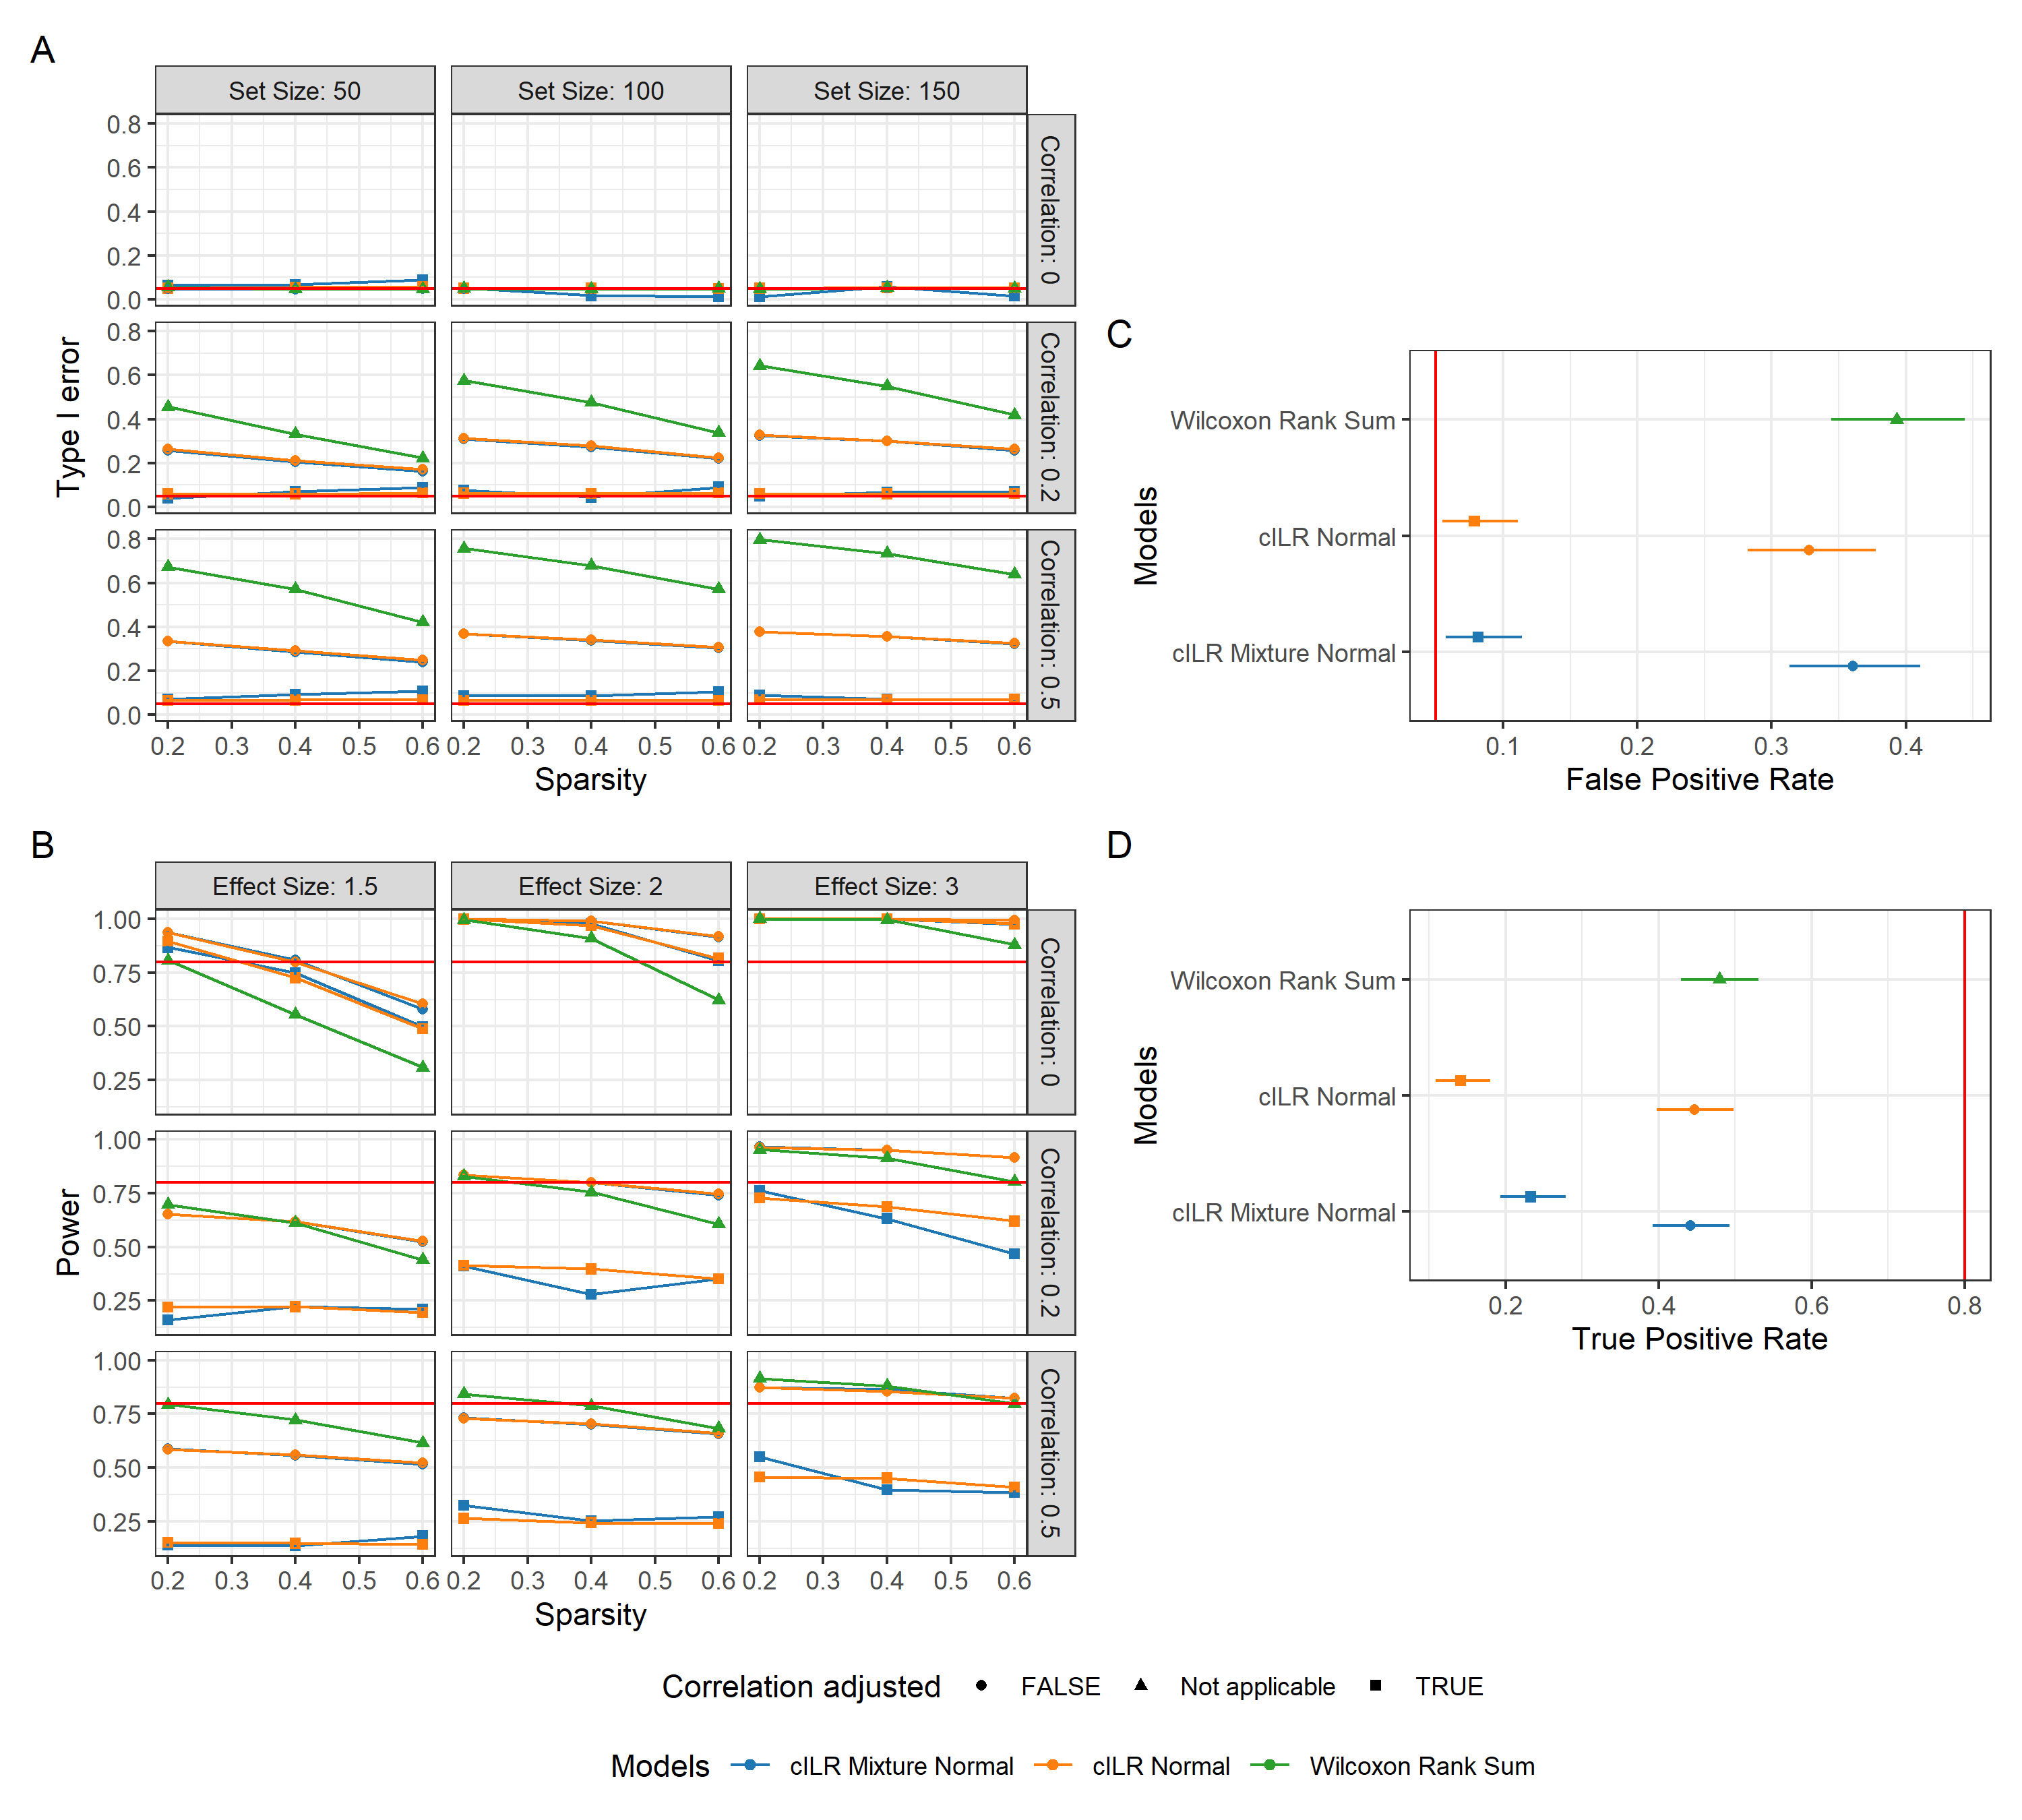
\includegraphics[width=\textwidth]{figures/sim_data_ss_hypo.png}
    \caption{Sample-level inference with CBEA under parametric simulations (\textbf{(A)} and \textbf{B}), and real data analysis (\textbf{(C)} and \textbf{(D)}). In simulation analyses, panel \textbf{(A)} shows type I error rate, and panel \textbf{(B)} shows power for single sample enrichment test for a specified set and was compared against a Wilcoxon rank sum test at $\alpha$ of 0.05. In real data analysis, panel \textbf{(C)} shows the false-positive rate, and panel \textbf{(D)} shows the true positive rate. For this analysis, 16S rRNA data from the oral microbiome of the gingival site was used. The set of aerobic microbes was tested for enrichment in all samples and was identified as correctly enriched if a significant $p$-value was obtained in supragingival samples. Confidence bounds were obtained using Agresti-Couli \cite{agresti1998} approach. Adjusted CBEA demonstrated control of type I error at the appropriate $\alpha$ level while remaining methods (not included in subsequent power analyses) showed an inflated type I error rate. However, this resulted in lower power for adjusted CBEA methods.}
    \label{fig:2}
\end{figure}

\subsection{Power analyses}
However, the trade-off for good type I error control is demonstrably lower power, as shown in Fig~\ref{fig:2}B. In situations where there is no inter-taxa correlation, CBEA still outperforms the wilcoxon rank sum test, however adjusted versions of CBEA did not perform as well as un-adjusted ones. However, in higher correlation scenarios, the difference in power is much more dramatic. At the highest effect size (fold change of 3) and correlation ($\rho = 0.5$), adjusted CBEA was only performing at 50\% power, while unadjusted CBEA and wilcoxon rank sum test were able to reach 80\%. These results indicate that both sparsity and inter-taxa correlation impacts power, with correlation having a much more dramatic impact especially for adjusted versions of CBEA. Most importantly, CBEA demonstrate higher power in all scenarios where type I error is properly controlled.    

To further assess the utility of CBEA in classifying samples with enriched sets, we generated AUC scores for different CBEA scores using true labels of whether a sample has an inflated set. This analysis, therefore, assessed the relative ranking of samples using CBEA scores whereby high scores should correspond to samples that are known to be inflated. Fig~\ref{fig:3} presents this result. We compared different variants of CBEA against competing methods in the gene set testing space (GSVA \cite{hanzelmann2013} and ssGSEA \cite{barbie2009}), as well as the $W$ test statistic from the Wilcoxon rank sum test. Across both simulations (Fig~\ref{fig:3}A) and real-data applications (Fig~\ref{fig:3}B), CBEA scores perform marginally better especially in low effect size situations but did not stand out in most other scenarios. In simulation studies, classification performance was good (around AUC of 0.8) even at high correlation settings, only requiring medium effect sizes (fold change of 2). Notably, the W-statistic provided the least information for classifying samples with inflated taxa.

\subsubsection*{Real data evaluations}  
These observations were replicated when assessed on the semi-labeled gingival data set from the Human Microbiome Project as described in \nameref{methods}. Here, we tested the enrichment of aerobic microbes for each sample using approaches similar to our parametric simulations. As expected in Fig~\ref{fig:2}C, the proportion of falsely rejected hypotheses was high in the naive Wilcoxon test and unadjusted CBEA methods. Conversely, adjusted CBEA controls for false positives adequately at the correct $\alpha$ level of 0.05. Power analysis (Fig~\ref{fig:2}D) showed similar patterns, where unadjusted CBEA methods and the Wilcoxon test have a higher proportion of null hypotheses correctly rejected, however, these results are not useful to a practitioner as the number of falsely rejected hypotheses are also equally high.